\chapter{Introduction}
\label{chap:Introduction}

		\section{Transport and confinement}
		\label{sec:TransportEtConfinement}

The performances of a reactor can be assessed with the help of several quantities. For example, from an economic point of view, the most often used is the ratio of the power produced by a plant to the power provided by the operator. This criterion must take into account the conversion losses (from the thermal power of the fusion products to the thermal power of a turbine and to the electrical power delivered by the plant to the grid). From the plasma physics point of view, which will be ours in these lecture notes, a more interesting efficiency criterion will be the ratio of the power produced by the fusion reactions to the external power absorbed by the plasma (ohmic heating, neutral beam and wave heating). There are other comparisons useful to assess and improve a fusion plant: the ratio of the plasma facing component lifetime to the plant lifetime, etc.

The ratio used in plasma physics is generally denoted $Q$:

\[
Q = \frac{P_{fus}}{P_{ext}}
\]

The $Q$ factor is really useful only in the very few experiments where tritium is used as a fuel. It was the case in TFTR, in which the last experimental campaign was dedicated to the study of a fusion plasma made of a 50-50 mix of deuterium and tritium. It is also the case in JET, where two trace tirtium experiments have been performed.

To assess the performances of a present day tokamak plasmas, almost always made of deuterium only, it is more relevant to evaluate the residence time of the energy providedd to the plasma. When this power is 'not too high' (we will come back to this threshold idea several times in these notes) the spontaneous organisation of the plasma is qualified as 'L mode' (for low confinement). A comparison the confinement times in a large number of experimental situations (different geometry, plasma current, density, etc.) corresponding to this mode, a scaling law was established. It is a power law of the confinement time as a function of several physical quantities. The L-mode scaling law based on the largest database, called the ITER89-P law, is the following:
\[
\tau_E^{ITER89-P} = 0,048 \frac{I^{0,85}R^{1,2}a^{0,3}\kappa^{0,5}(n/10^{20})^{0,1}B^{0,2}A^{0,5}}{P^{0,5}}
\]
where $I$ (in MA) is the plasma current, $R$ and $a$ are the major and minor radii respectively, $\kappa$ the elongation (major axis to minor axis ratio of a poloidal cross section), $n$ the electron density, $B$ the magnetic field, $A$ the fuel ion mass number and $P$ (in MW) the injected power.

The discovery of a more favourable organisation mode in the 1980s, the H mode ('high confinement'), and the need for quantifying the improvement it brings, led to the elaboration of another scaling law:
\[
\tau_E^{IPB98(y,2)} = 0,145 \frac{I^{0,93}R^{1,39}a^{0,58}\kappa^{0,78}(n/10^{20})^{0,41}B^{0,15}A^{0,19}}{P^{0,69}}.
\]

In practice, the comparison between a particular experiment and a reference is based on the scaling laws.A new factor, denoted H, has thus been defined. It is the ratio of the experimentally determined confinement time $\tau_E^{exp}$ in such a scenario to the $\tau_E$ predicted by the L-mode scaling law:
\[
H = \frac{\tau_E^{exp}}{\tau_E^L}.
\] 
We use also the comparison to the H-mode scaling law: $H_{IPB98} = \tau_E^{exp} / \tau_E^{IPB98(y,2)}$. The higher the H factor, the better the energy confinement.

There are other favourable confinement modes, although they are less well known and controlled. They are called 'internal transport barriers or ITB because they are characterised by an innner plasma region where confinement is substantially better than elsewhere in the plasma. The performances of these modes are also assessed with the H factor.

As the reader will have noticed, the H factor allows a global evaluation of the plasma performance. It does not give information on the localisation or the volume fraction which is responsible for the confinement, or the physics phenomena which drive the energy exchanges between the various plasma regions. If the physicists want to play an active role in the improvement of a fusion plant or conception of a new machine, they must have look for a more detailed description of the energy exchanges in the plas with the help of diffusive models or others. This is what we call generically transport studies.

Transport processes do not concern only energy. The plasma particles, which carry this energy, are submitted to forces which drive their motion in the plasma: electrostatic force, Lorentz force, etc., which determine the particle lifetime in the plasma. The macroscopic result of particle transport is reflected in the (electron and ion) density profile shape, which itself acts directly on the fusion reaction rate.

Finally, the performances of a fusion plasma are determined bby the plasma temperature, which depends on the externally provided power bu also on the power exhaust processes. Radiation by charged particles, which increases with the particle charge, is the main cause of power losses. It is thus essential to minimise fuel contamination by impurities. Hence the need to control impurity transport as well. Among these impurities, one plays a peculiar role: the helium nuclei produced by the fusion reactions (alos called $\alpha$'s). They must stay in the plasma long enough for their kinetic energy to be damped, and short enough once thermalisednot to contribute to fuel dilution and radiated power losses. Helium transport studies, although difficult in their experimental aspects, should become a priority in the next few years.

The theory of transport in tokamak plasmas is still evolving. An introduction to the subject will be found in references \cite{cea1987, wesson2004, chen2006}. More detailed discussions about transport associated with collisions can be found in \cite{hinton1976, hirshman1981, helander2002}. Many articles on turublent transport but up to now none gives a complete overview of hte subject.




		\section{Framework: diffusive-convective transport}
		\label{sec:CadreDeTravail}

%Sources bibliographiques: 

%N.J. Lopes Cardozo, \textit{Perturbative Transport Studies in Fusion Plasmas}, \textsc{Plasma Phys. Control. Fusion 37 (1995)799-852.}
		
				\subsection{A generic transport model}
				\label{sub:ModeleGeneriqueDeTransport}
				
						\subsubsection{Model definition}
						\label{subsub:DefinitionDuModele}
						
Several physics models allow to express a heat flux, a particle flux or a momentum flux as a function of the plasma quantities: density, temeprature, angular momentum. Some of these models will be detailed later in these notes but some information about transport can be drawn from very general considerations on the flux expressions and their evolution equations.

In most models, the heat and particle fluxes have the following form:
\begin{eqnarray}
	\vec{q} 			& = & -\chi n \vec{\nabla} T	\\
	\vec{\Gamma} 	& = & -D \vec{\nabla} n + \vec{V} n
\end{eqnarray}
where $\vec{q}$ and $\vec{\Gamma}$ denote a heat flux and a particle flux respectively (carried by electrons, ions or an impurity). In these expressions $\chi$, $D$ and $V$ represent a heat diffusion coefficient (or diffusivity), a particle diffusion coefficient and a convection velocity.

In general these vector expressions can be written in a simpler way. Indeed, the sole effect of the toroidal and poloidal components of the fluxes is ti homogenise particle and energy distributions on the flux surfaces. On the contrary the radial component drives matter and energy exchanges between flux surfaces of differnet radii. It is thus the only one which we will be interested in in our transport and confinement studies. In the following, the expressions related to the fluxes will be radial projections of the more general vector equations.

As a complement to these definitions, we will use the evolution equations for matter and energy (momentum can also be considered). The following expressions can be used:
\begin{eqnarray}
	\frac{\partial n}{\partial t}	+ \nabla. \Gamma  =  S_p	\\
	\frac{\partial}{\partial t} \left( \frac{3}{2}nT \right) + \nabla. q	+ \nabla. \left( \frac{5}{2}T\Gamma \right) - \frac{1}{n} \Gamma. \nabla \left(nT\right)	=  S_h
	\label{eq:Evolution}
\end{eqnarray}

The second on is sometimes written in a different form, using $\Gamma = nV$ and $p = nT$:
\[
\frac{3}{2} \left( \frac{\partial}{\partial t} + V.\nabla \right)p + \frac{5}{2}p\nabla.V + \nabla.q = S_h
\]

						\subsubsection{Properties of the model}
						\label{subsub:ProprietesDuModele}


Without expliciting the hysics phenomena which will allow to give a form to the transport coefficients (diffusioncoefficient and convection velocity) the generic model provides interesting information on transport.

\begin{quotation}
\textsc{Exercise:} Let us consider a sationary plasma: $\partial n / \partial t = 0$. In the plasma core in general there is no particle source (this is the simple case where the particle source is due to gas injection): $S_p = 0$. Give the analytical solution of the continuity equation in cylindrical coordinates (the coordinate system closest to the toric geometry of tokamaks). This solution gives a relation between the density gradient and the particle transport coefficients:
\[
	\frac{\nabla n}{n} = \frac{V}{D}
\]

\end{quotation}

The density profile shape depends on the transport coefficient ratio. Note that $V$ can be either positive or negative (i.e. outward or inward directed, adopting the mathematical convention for the $V$ sign), which correspondss to a peaked profile (the maximum is in the plasma centre) or a hollow profile (the maximum is at a radius $r$ different from 0), as illustrated in Fig. \ref{fig:Sens_piquage}.
\begin{figure}[htbp]
	\centering
		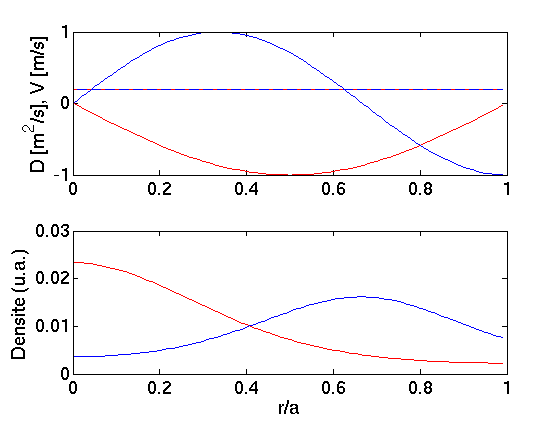
\includegraphics[width=0.70\textwidth]{Fig_Sens_piquage.png}
	\caption{Top: two cases of convection velocity radial profiles (for clarity, we have chosen identical, flat diffusion coefficient profiles indicated bi the two-colors line). Bottom: resulting density profiles in stationary states. The velocity direction has an influence on the density profile shape. When the velocity is negative (inward, red curves), the density profile is peaked. When the velocity is positive (outward, blue curve), the profile is hollow.}
	\label{fig:Sens_piquage}
\end{figure}

The same comment could be made for the temperature profile when using the heat transport equation but in general the heat sources are distributed in the plasma, which does not allow to solve the problem without a specific model.	

It is to be noticed that in the stationary case, the density profile measurement is not enough to determine separately $D$ and $V$. This determination can be done only by studying a transient state.

The difference between the study of a stationary state and that of a transient state is at the basis of heat transport experiments. Let us look again at the generic heat flux expression:

	\[
	q_e = -n_e\chi \nabla T_e
\]
Formally, the diffusivity can be deduced from the heat flux and temperature gradient measurements:
	\[
	\chi = -\frac{q_e}{n_e \nabla T_e}
\]
In practice, $\chi$ is in general a function of other gradients (which corresponds to non diagonal terms in the transport matrix, as will be seen in the next section). By isolating te term which depends only on $\nabla T_e$, we can write:
	\[
	q_e = -n_e\chi_e\nabla T_e + q_{offset} \mbox{, where } q_{offset} = \sum{M_{ij}\nabla u_j}
\]
In the case of a stationary plasma, we can deduce from the measurements:
	\[
	\chi_{stat} = -\frac{q_e}{n_e\nabla T_e} = \chi_e - \frac{q_{offset}}{n_e \nabla T_e}
\]
and in the case of a transient:
	\[
	\chi_{tr} = - \frac{\partial q_e}{n_e \partial \left( \nabla T_e\right)} = \chi_e
\]

The coefficients determined by these two methods are different, although they both represent a diffusivity. The difference between the two contains information on the dependence of diffusivity in other gradients of the plasma. The role of these other gradients must be investigated with speific experiments.
				
				
				\subsection{Transport matrix}
				\label{sub:MatriceDeTransport}

The flux expressions as functions of the associated plasma quantities suggest a matrix-like writing:
				
\[
	\Phi = M \nabla U
\]
where $\Phi$ is flux vector and $U$ is the vector of the associated plasma quantities. Let us take as an example the simple case where only the electron particle and heat fluxes are considered: 

	\[
	\Phi = \left(
								\begin{array}{c}
									q_e				\\
									\Gamma_e
								\end{array}
				 \right)
	\mbox{, }
	U =		\left(
								\begin{array}{c}
									T_e				\\
									n_e
								\end{array}
				 \right)
\]
but a more complete and detailed matrix can be built with the heat and particle fluxes for electrons, ions and the various types of impurities involved in the case under study.

The diagonal elements of this matrix are the diffusion coefficients (multiplied by density for the heat part). If for instance  electrons, ions and an impurity species are to be studied, one will have: 
	\[
	\Phi = \left(
								\begin{array}{c}
									q_e				\\
									q_i				\\
									q_Z				\\
									\Gamma_e	\\
									\Gamma_i	\\
									\Gamma_Z
								\end{array}
					\right)
		\mbox{, }
		U = \left(
								\begin{array}{c}
									T_e				\\
									T_i				\\
									T_Z				\\
									n_e				\\
									n_i				\\
									n_Z
								\end{array}
				 \right)
\]
and the transport matrix diagonal will be:
	\[
	M_{diag} = 	\left(
								\begin{array}{cccccc}
									-n_e\chi_e	&				0			&				0			&		0		&		0		&		0		\\
											0				&	-n_i\chi_i	&				0		 	& 	0 	&		0		&		0		\\
											0				&				0			&	-n_Z\chi_Z	& 	0 	&		0		&		0		\\
											0				&				0			& 			0			&	-D_e	&		0		&		0		\\
											0				&				0			&				0			&		0		&	-D_i	&		0		\\
											0				&				0			&				0			&		0		&		0		&	-D_Z
								\end{array}
							\right)
\]

We will see later that the convection velocity of a given impurity type caused by binary particle collisions depends on gradients:
	\[
		\Gamma_Z = -D_Z \left[	
													\nabla n_Z - \left(	
																					\frac{ \nabla n_i}{n_i} + ZH_Z \frac{\nabla T_i}{T_i}
																			 \right) n_Z
										\right]
\]
These dependences will be included in the transport matrix in the form of non diagonal terms.

In order to obtain simple flux expressions with only diffusion-like terms (i.e. in the form $\Phi = -D\nabla U$),we can diagonalise the transport matrix. The eigenvector basis in which it is diagonal is a linear combination of physical states. For instance, if we are interested in a situation where only the electron heat and particle fluxes must be taken into account, the basis iin which the matrix is diagonal will be made of linear combinations of $T_e$ and $n_e$. The eigen states thus do not have a clear physical meaning. To each eigenstate is associated an eigenvalue wich is the time constant characteristic of the eigenstate evolution. Conversely, each physical quantity is a linear combination of the eigenstaes. It is thus characterised by several time constants. This somewhat abbstract observation has been done also on experimental results.

Finally, there also exist terms (such as the convection velocity due to the Ware effect) which do not depend on the gradients. They are introduced on the transport matrix in a somewhat artificial way, a consequence of which is that the transport matrix is not unique.

As we have seen, the transport matrix, whose definition seems natural given the form taken by the fluxes in most theoretical models, is thus a delicate object as far as handling and interpetation are concerned. It can be useful since it allows to retrieve the characteristic time constants of a problem but it refers to quantities whose physical meaning is uncertain and abstract. 

				\subsection{Linearisation of the transport equations}
				\label{sub:LinearisationDesEquationsDeTransport}

The interest of transients for the experimental transport determination has been shown above. This is why transport experiments consist often in perturbing a stationary plasma state by a heat pulse or a particle injection. To reveal the type of transport which governs the stationary state under study, these perturbations must be small. This is the framework in which we are going to exhibit more prooperties of the generic transport model.
	
If the stationary plasma state is weakly perturbed, the evolution equations of §\ref{subsub:DefinitionDuModele} can be rewritten using the following definitions:

\begin{eqnarray}
	n 			&	=	& n_{eq} + \tilde{n}	\nonumber	\\
	T 			&	=	& T_{eq} + \tilde{T}	\nonumber	\\
	\ldots	&		&											\nonumber	\\
	\Gamma	&	=	& \tilde{\Gamma}			\nonumber	\\	
	q 			&	=	& \tilde{q}						\nonumber	\\
	\ldots	&		&											\nonumber	\\
	S_p 		&	=	& \tilde{S_p}					\nonumber	\\
	S_h 		&	= &	\tilde{S_h}					\nonumber	\\
	\ldots	&		&											\nonumber
\end{eqnarray}
where $n_{eq}$ and $T_{eq}$ are the density and temperature of the stationary state, $\tilde{n}$ and $\tilde{T}$ are the associated fluctuations, and the same notations are used for the fluxes (to retain simple expressions, sources and fluxes are assumed to be 0 for the stationary states).

Without any assumption on the flux form (e.g. the particle flux may depend on density, temperature, etc. and their gradients), the perturbed particle flux can be written as:
\begin{eqnarray}
	\tilde{\Gamma} & = & \frac{\partial \Gamma}{\partial \left( \nabla n \right)}\nabla \tilde{n} + \nonumber	\\
								&		& \frac{\partial \Gamma}{\partial \left( \nabla T \right)}\nabla \tilde{T} + 
													\ldots  + \nonumber	\\
								&		& \frac{\partial \Gamma}{\partial n}\tilde{n} + \frac{\partial \Gamma}{\partial T}\tilde{T}
													+ \ldots
\end{eqnarray}
The first line represents the diagonal term (diffusion). The second line represents the dependence of the particle fluw on the graidents other than the density gradient, i.e. the non diagonal terms of the problem. The third line represents the convective terms. The ellipsis contains the dependences on other gradients (e.g. that of another type of particles).

In the same way, the perturbed heat flux can be expressed as:
\begin{eqnarray}
	\tilde{q} & = & \frac{\partial q}{\partial \left( \nabla T \right)}\nabla \tilde{T} + \nonumber	\\
								&		& \frac{\partial q}{\partial \left( \nabla n \right)}\nabla \tilde{n} + 
													\ldots  + \nonumber	\\
								&		& \frac{\partial q}{\partial T}\tilde{T} + \frac{\partial q}{\partial n}\tilde{n}
													+ \ldots
\end{eqnarray}
Taking into account these expressions, the evolution equations expressed in amatrix form become:
\begin{eqnarray}
	\frac{\partial}{\partial t} \left( \begin{array}{cc}
																				\tilde{n}	\\		
																				\tilde{T}
																		 \end{array}
															\right)
																			& = &	-\nabla \left(
																												\begin{array}{cc}
																														\tilde{\Gamma} \\
																														\tilde{q}
																												\end{array}
																										\right)
																						+ \left(
																									\begin{array}{cc}
																											\tilde{S_p}	\\
																											\tilde{S_h}
																									\end{array}
																							\right)				\nonumber		\\
																			& = & A \nabla^2 \tilde{U} + B \nabla \tilde{U} + C\tilde{U} + \tilde{S}
\end{eqnarray}
by writing: 
\[
\tilde{U} = \left( \begin{array}{cc} 
							\tilde{n} \\ 
							\tilde{T}  
					 \end{array} 
		\right) \mbox{ et } 
\tilde{S} = \left( \begin{array}{cc}
							\tilde{S_p} \\ 
							\tilde{S_h} 
					 \end{array} 
		\right)\mbox{.}
\] 

The first term corresponds to diffusion, the second one to convection, the third is a damping term (if the C coefficients are negative). Note that $A$, $B$ and $C$ are matrices which contain the flux dependences on the plasma quantities and their gradients. Fro instance, the matrix elements of $A$ cna be easily calculated:

\[
\begin{array}{ll}
		A_{11} = \frac{\partial\Gamma}{\partial (\nabla n)}		&		A_{12} = \frac{T_{eq}}{n_{eq}} \frac{\partial\Gamma}{\partial(\nabla T)}		\\
		A_{21} = \frac{2}{3}\left( \frac{\partial\Gamma}{\partial (\nabla n)} + \frac{1}{T_{eq}}\frac{\partial q}{\partial (\nabla n)} \right)													&  A_{22} = \frac{2}{3}\left( \frac{1}{n_{eq}}\frac{\partial q}{\partial (\nabla T)} + \frac{T_{eq}}{n_{eq}}\frac{\partial\Gamma}{\partial\nabla T} \right)
\end{array}
\]

The diagonal coefficients $A_{11}$ and $A_{22}$ correspond to the heat and particle diffusion coefficients (with a $n_{eq}$ factor for the former), as already said.

We can deduce a few properties from this result. An example will be given now. Let us consider the simple case of an experiment where only one quantity is perturbed, excluding all others. The transport matrix is reduced to only one line. Let us assume in addition that we are in a purely diffusive case in one dimension. The only evolution equation is thus:

\[
	\frac{\partial u}{\partial t} = -D \frac{\partial^2 u}{\partial x^2}
\]
In the case of a sine-like periodic perturbation, the boundary conditions are:
\[
\begin{array}{ll}
		u(x=0,t) = u_0 e^{i\omega t} \\
		u(\infty, t) = 0
\end{array}
\]
the solution of this equation is:
\[
	u = u_0 e^{-x/\lambda}e^{i(\omega t - kx)}
\]
The complete resolution shows that the characteristic decay length and the phase velocity of the perturbation are:
\begin{eqnarray}
	\lambda = \sqrt{\frac{2D}{\omega}}	\nonumber	\\
	v_\phi = \sqrt{2\omega D}						\nonumber	
\end{eqnarray}

A high frequency (or fast) perturbation thus penetrates faster but shallower than a low frequency (or slow) perturbation. This property, among others, is used in the Fourier analysis method commonly used in heat transport studies.




